Die Wellenlängen der Dublettlinien werden mit Hilfe eines Gitterspektralapparates bestimmt (siehe Abbildung VERWEIS). Der Strahl der Lichtquelle -- hier Natrium, Kalium und Rubidium -- wird gebündelt und auf ein optisches Gitter fokussiert. Mit dem Fernrohr kann der gebrochene Strahl in Abhängigkeit des Brechungswinkels untersucht werden. \\
\begin{figure}[h!]
	\centering
	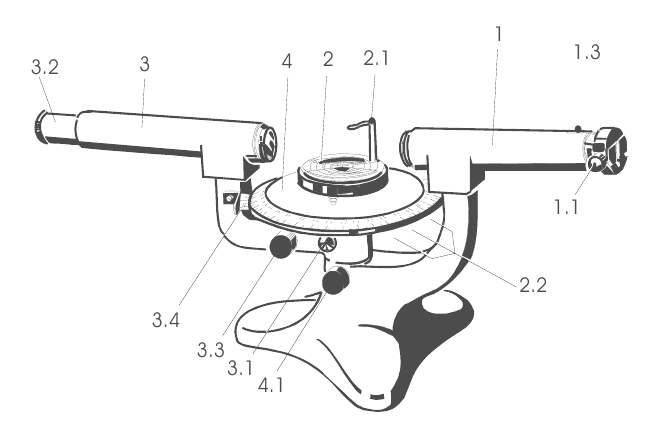
\includegraphics[width=0.8\textwidth]{Spektrometer.png}
	\caption{Aufbau eines Gitterspektrometers}
\end{figure}
Zunächst werfen die bekannten Spektrallinien der Helium-Quelle ausgemessen, um die Gitterkonstante der Apparatur zu bestimmen. Bei dem Transmissionsgitter muss zunächst die Achse des transmittierten Stahls d.h. des nullten Hauptmaximums notiert werden, um die Differenzen zum jeweils nächsten Maximum ermitteln zu können. \\
Für die Vermessung der Dublettlinien wird  eine höhere Genauigkeit benötigt, die durch ein Okularmikrometer erreicht wird -- eine Mikrometerskala, die ins Blickfeld des Fernrohrs eingebaut ist.

